\begin{tikzpicture}
    %Pre-filter
    \draw[->] (-6,0)node[anchor=east]{$\dot{Q}_{HEX}$} -- (-4,0);
    \draw (-4,-0.5) rectangle (-3,0.5) node[pos=0.5]{$F(s)$};
    %Sum
    \draw[->] (-3,0) -- (-2,0) node[pos=0.5,anchor=south]{$\dot{Q}_{Core}^{SP}$};
    \draw (-1.75,0) circle (0.25) node{\scriptsize$-$};
    %Controller
    \draw[->] (-1.5,0) -- (-0.5,0)node[pos=0.5,anchor=south]{$e(s)$};
    \draw (-0.5,-0.5) rectangle (0.5,0.5) node[pos=0.5]{$C(s)$};
    \draw[->] (0.5,0) -- (1.5,0) node[pos=0.5,anchor=south]{$u(s)$};
    %Actuator
    \draw (1.5,-0.5) rectangle (2.5,0.5) node[pos=0.5]{$A(s)$};
    \draw[->] (2.5,0) -- (3.5,0);
    \draw[red,very thick] (2,0) circle (0.8);
    \draw[->,red,thick] (-2,-2) -- (1.4,-0.6);
    \draw[->,red,thick] (6,-2.2) -- (2.6,-0.6);
    %Process
    \draw (3.5,-0.5) rectangle (4.5,0.5) node[pos=0.5]{$P(s)$};
    \draw[->] (4.5,0) -- (6.5,0) node[anchor=west]{$\dot{Q}_{Core}$};
    %Transducer
    \draw[->] (5.5,0) -- (5.5,-1.5) -- (2.5,-1.5);
    \draw (1.5,-2) rectangle (2.5,-1) node[pos=0.5]{$H(s)$} ;
    \draw[->] (1.5,-1.5) -- (-1.75,-1.5) -- (-1.75,-0.25);
    %Passive Feedback
    \draw[->] (5.5,0) -- (5.5,1.5) -- (4.5,1.5);
    \draw[->] (-5,0) -- (-5,1.5) -- (3.5,1.5);
    \draw (3.5,1) rectangle (4.5,2) node[pos=0.5]{$G(s)$};
    \draw[->] (4,1) -- (4,0.5);

    \node at (-4,-3) {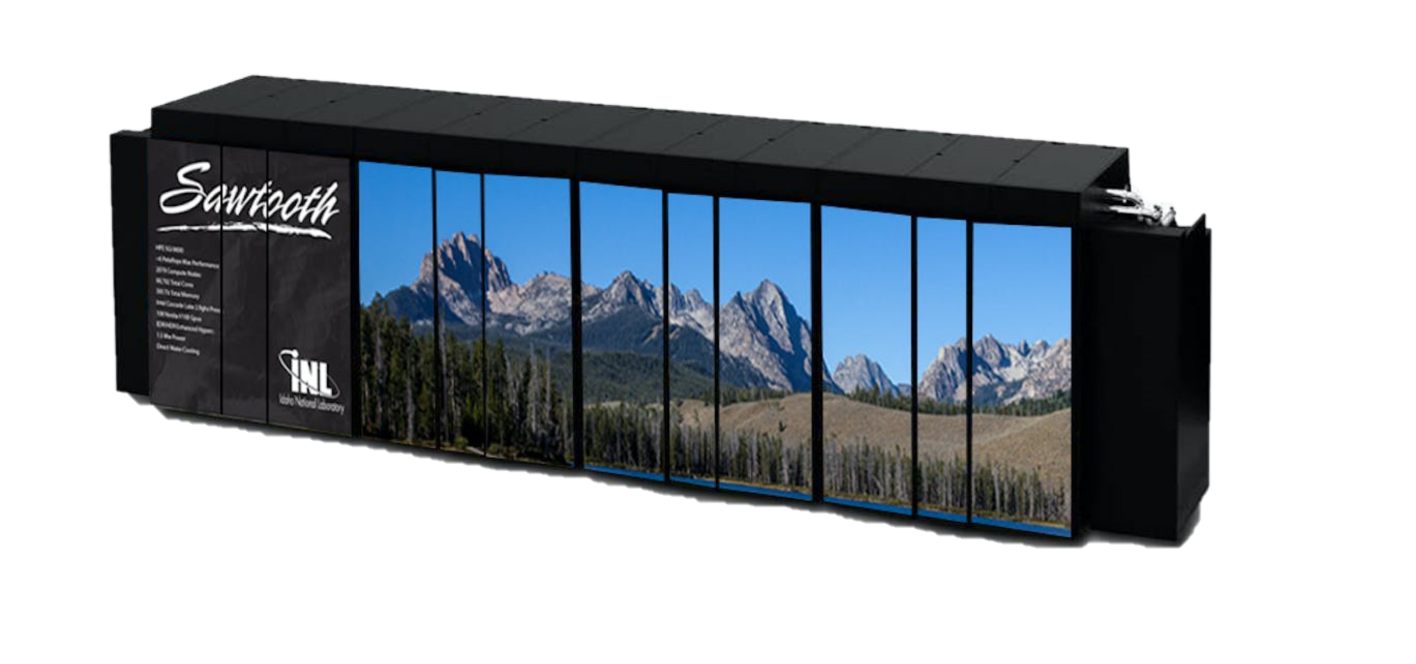
\includegraphics[height=3.5cm]{sketch/Sawtooth}};
    \node at (4.5,-3.5) {
\includegraphics[height=2.5cm]{sketch/serpent}};
\end{tikzpicture}